


\documentclass[a4paper,12pt,spanish]{article}

\usepackage[utf8]{inputenc}


\usepackage{blindtext}
%\usepackage{microtype}
\usepackage{amsfonts, amsmath, amsthm, amssymb}
%\usepackage{fancyhdr}
%\usepackage{index}
%\usepackage{multicol}    

%\usepackage{booktabs}

\usepackage[T1]{fontenc}
\usepackage[utf8]{inputenc}
\usepackage{graphicx}
\usepackage[spanish,es-tabla]{babel}
\usepackage{url}
\usepackage{enumitem}

\usepackage[unicode=true, pdfusetitle,
bookmarks=true,bookmarksnumbered=false,bookmarksopen=false,
breaklinks=true,pdfborder={0 0 1},backref=false,colorlinks=false]
{hyperref}

\usepackage{listings}
\usepackage{longtable}


\usepackage{siunitx} %para el sistema internacional
\usepackage[export]{adjustbox}
\usepackage{booktabs} 
\usepackage{subcaption}

\usepackage{float}


\newcommand{\address}[1]{
	\par {\raggedright #1
		\vspace{1.4em}
		\noindent\par}
}

\usepackage[table,xcdraw]{xcolor}


\pagenumbering{gobble}
\include{noNumberPage}
\pagenumbering{arabic}
\setcounter{page}{1}

%tutorial de tablas latex: https://manualdelatex.com/tutoriales/tablas

\usepackage{multirow}

% \usepackage[table,xcdraw]{xcolor}


%Inicio del documento (hasta que se cierre con \end{document}
\begin{document}
	
	
	\title{ Relación de dispersión de ondas de tensión superficial}
	
	%\author{Adrián Rivero Fernández}
	\date{}
	
	\maketitle
	
	
	\section{Objetivos de la práctica}
	
	En esta práctica determinaremos experimentalmente la tensión superficial de un líquido a partir de la relación de dispersión de ondas de tensión superficial
	
	\section{Resumen teórico}
	
	%[Escribirlo cuando tengamos un poco más claro qué usamos dentro de esta práctica]
	
	Al producirse una perturbación en un fluido, de modo que un elemento de volumen se desplaza fuera de su posición de equilibrio, actúan como fuerzas recuperadoras la fuerza de la gravedad y la tensión superficial, generando cada una un tipo de onda asociada. El orden de magnitud de la fuerza recuperadora generada por la gravedad corresponde a $\rho\cdot g$ (siendo $\rho$ la densidad del fluido y $g$ la gravedad). La fuerza generada por la tensión tiene una magnitud de $\sigma \cdot k$ (siendo $\sigma$ la tensión superficial y $k$ el número de onda $k = 2\pi / \lambda$ con $\lambda$ siendo la longitud de onda).\\
	
	La denominada relación de dispersión representa la relación entre el número de onda $k$ y la frecuencia angular $\omega$, que depende del medio y de las fuerzas involucradas en el proceso. A partir de linealizar las ecuaciones de Navier-Stokes y de la ecuación de Young-Laplace, obtenemos que
	\[ \omega^2(k) = \frac{\sigma}{\rho} k^3
	\]
	
	Esta relación se puede obtener experimentalmente para ondas de tensión superficial estacionarias en la superficie de un líquido, a partir del patrón de difracción de la incidencia de un haz de luz monocromática en la superficie. Podemos inducir una perturbación de frecuencia sobre el líquido, excitando un modo normal de vibración para generar las ondas estacionarias, iluminarlas con un haz de luz y obtener reflejos sobre una pantalla que muestren un patrón de difracción que nos de información sobre los puntos en los que se ha producido interferencia constructiva.
	
	
	
\begin{figure}[H]
	\centering
	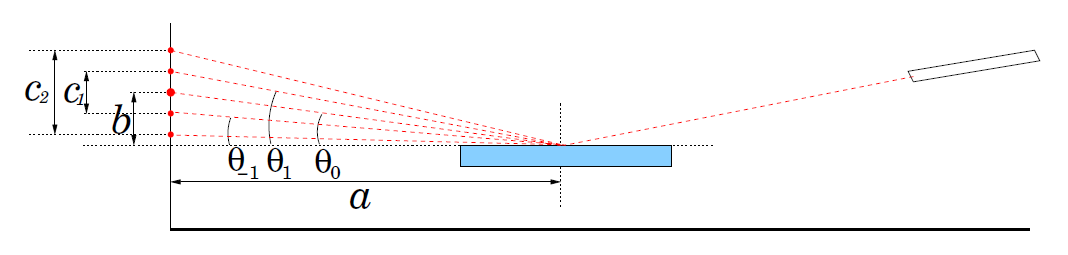
\includegraphics[width=\linewidth]{../fotos/image.S8OFM2}
	\caption{Esquema del patrón de difracción}
	\label{fig:image}
\end{figure}
	
	La Figura \ref{fig:image} representa el esquema del patrón de difracción de las ondas reflejadas en una superficie con ondas de tensión superficial estacionarias. $\theta_0$ es el ángulo del máximo principal, $\theta_1$ y $\theta_{-1}$ son los de los máximos secundarios de primer orden. La distancia $a$ es la distancia del punto de reflexión a la pantalla, $b$ es su altura relativa, y $c_1$ y $c_2$ es la distancia entre máximos secundarios.
	
	
	A partir de los ángulos de los máximos secundarios y central de los puntos luminosos, podemos obtener el número de onda:
	\[ k_n = \frac{\pi}{n\lambda}(\theta_n - \theta_{-n})\sin\theta_0
	\]
	que para ángulos pequeños puede aproximarse como 
	\[ k_n = \frac{\pi}{\lambda}(\theta_n - \theta_{-n})\theta_0
	\]
	
	Siendo $c_n$ la distancia entre máximos secundarios de orden $n$, podemos aproximar 
	\[(\theta_n - \theta_{-n}) = \frac{c_n}{a}
	\]
	De modo que 
	\[ k_n = \frac{\pi}{n \lambda} \theta_0 \frac{c_n}{a}
	\]
	
	%=P5/G5*H5+P5/(M5/1000)*(1/1000) + (2*P5/$B$2)*$B$3+ (P5/$B$5)*$B$6
	
	
	
	
	\section{Procedimiento experimental}
	
	Mediante el transmisor mecánico acoplado a un altavoz, conectado a un generador de señales, generaremos una onda estacionaria de tensión superficial en agua destilada. Haremos incidir el haz de luz láser sobre la superficie, en el punto en el que se genera la onda estacionaria. Esta superficie actúa como una red de difracción. Haremos que se refleje en una pantalla para ver su patrón, en el que identificaremos un máximo central y dos secundarios de primer y segundo orden.


\begin{figure}[H]
	\centering
	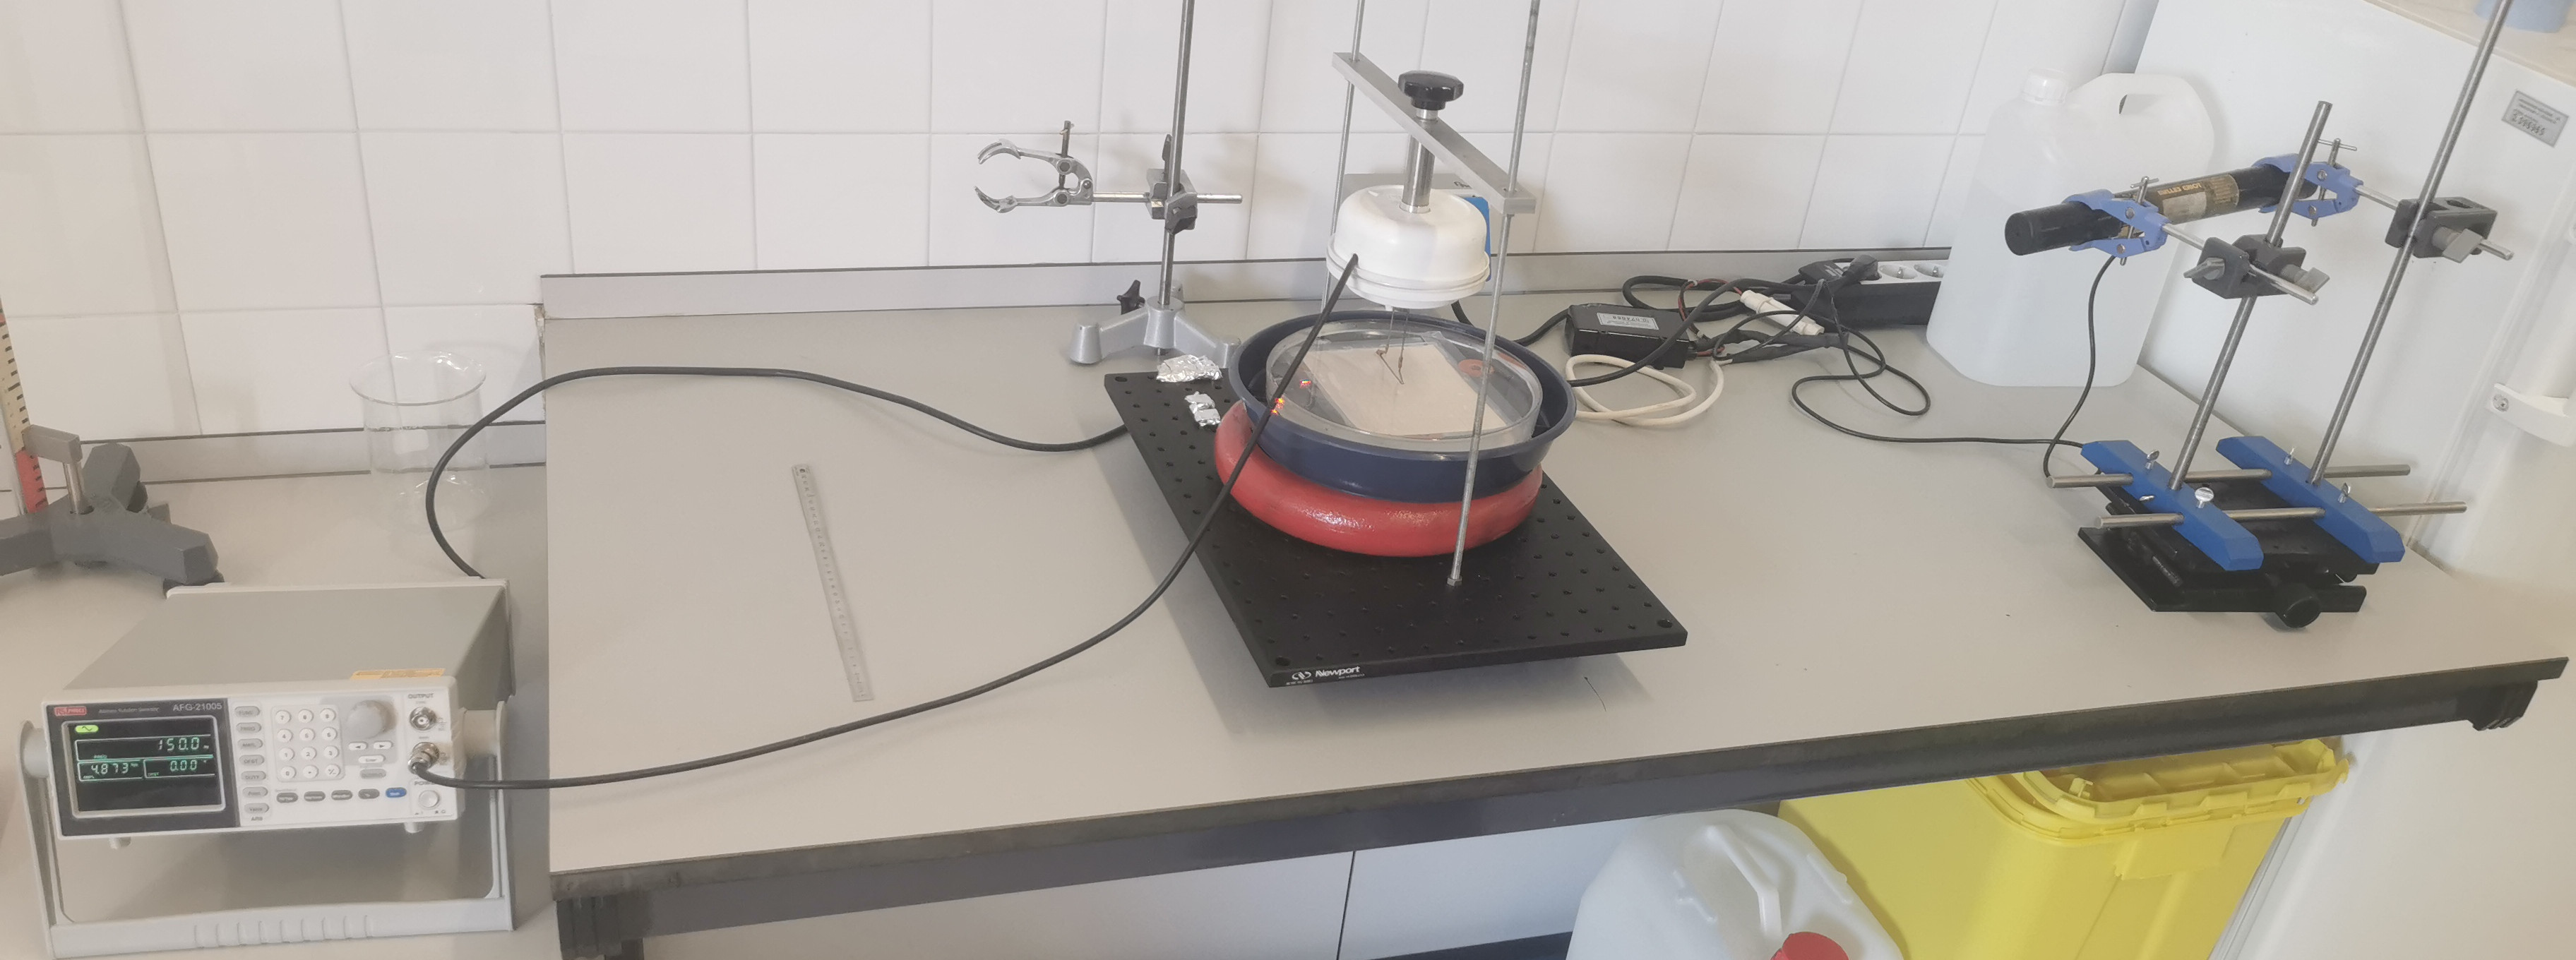
\includegraphics[width=0.9\linewidth]{../fotos/IMG_20240307_101213-r}
	\caption{Dispositivo experimental}
	\label{fig:img20240307101213-r}
\end{figure}
	
	\subsection*{Procedimiento}
	
	\begin{enumerate}
		\item Llenamos el recipiente con agua destilada y medimos su temperatura.
		
		\item Establecemos contacto entre el transmisor mecánico y la superficie del agua. El segmento horizontal debe contactar paralelamente con la	superficie del líquido quedando parcialmente sumergido. Modificaremos la altura del transmisor mecánico y lo nivelaremos respecto a la superficie actuando sobre	las tuercas que sujetan el soporte, donde se encuentra anclado.
		
		\item Ajustamos el haz de luz láser de modo que su reflejo en la superficie del agua es visible en la pantalla. Observamos, en ausencia de perturbación, un punto estático en la pantalla.
		
		\item Conectamos el generador de señales. Seleccionamos una frecuencia entre 150 y 400 Hz. La vibración generará ondas estacionarias en la superficie.
		
		\begin{figure}    %ojo que esto está sin fijar
			\centering
			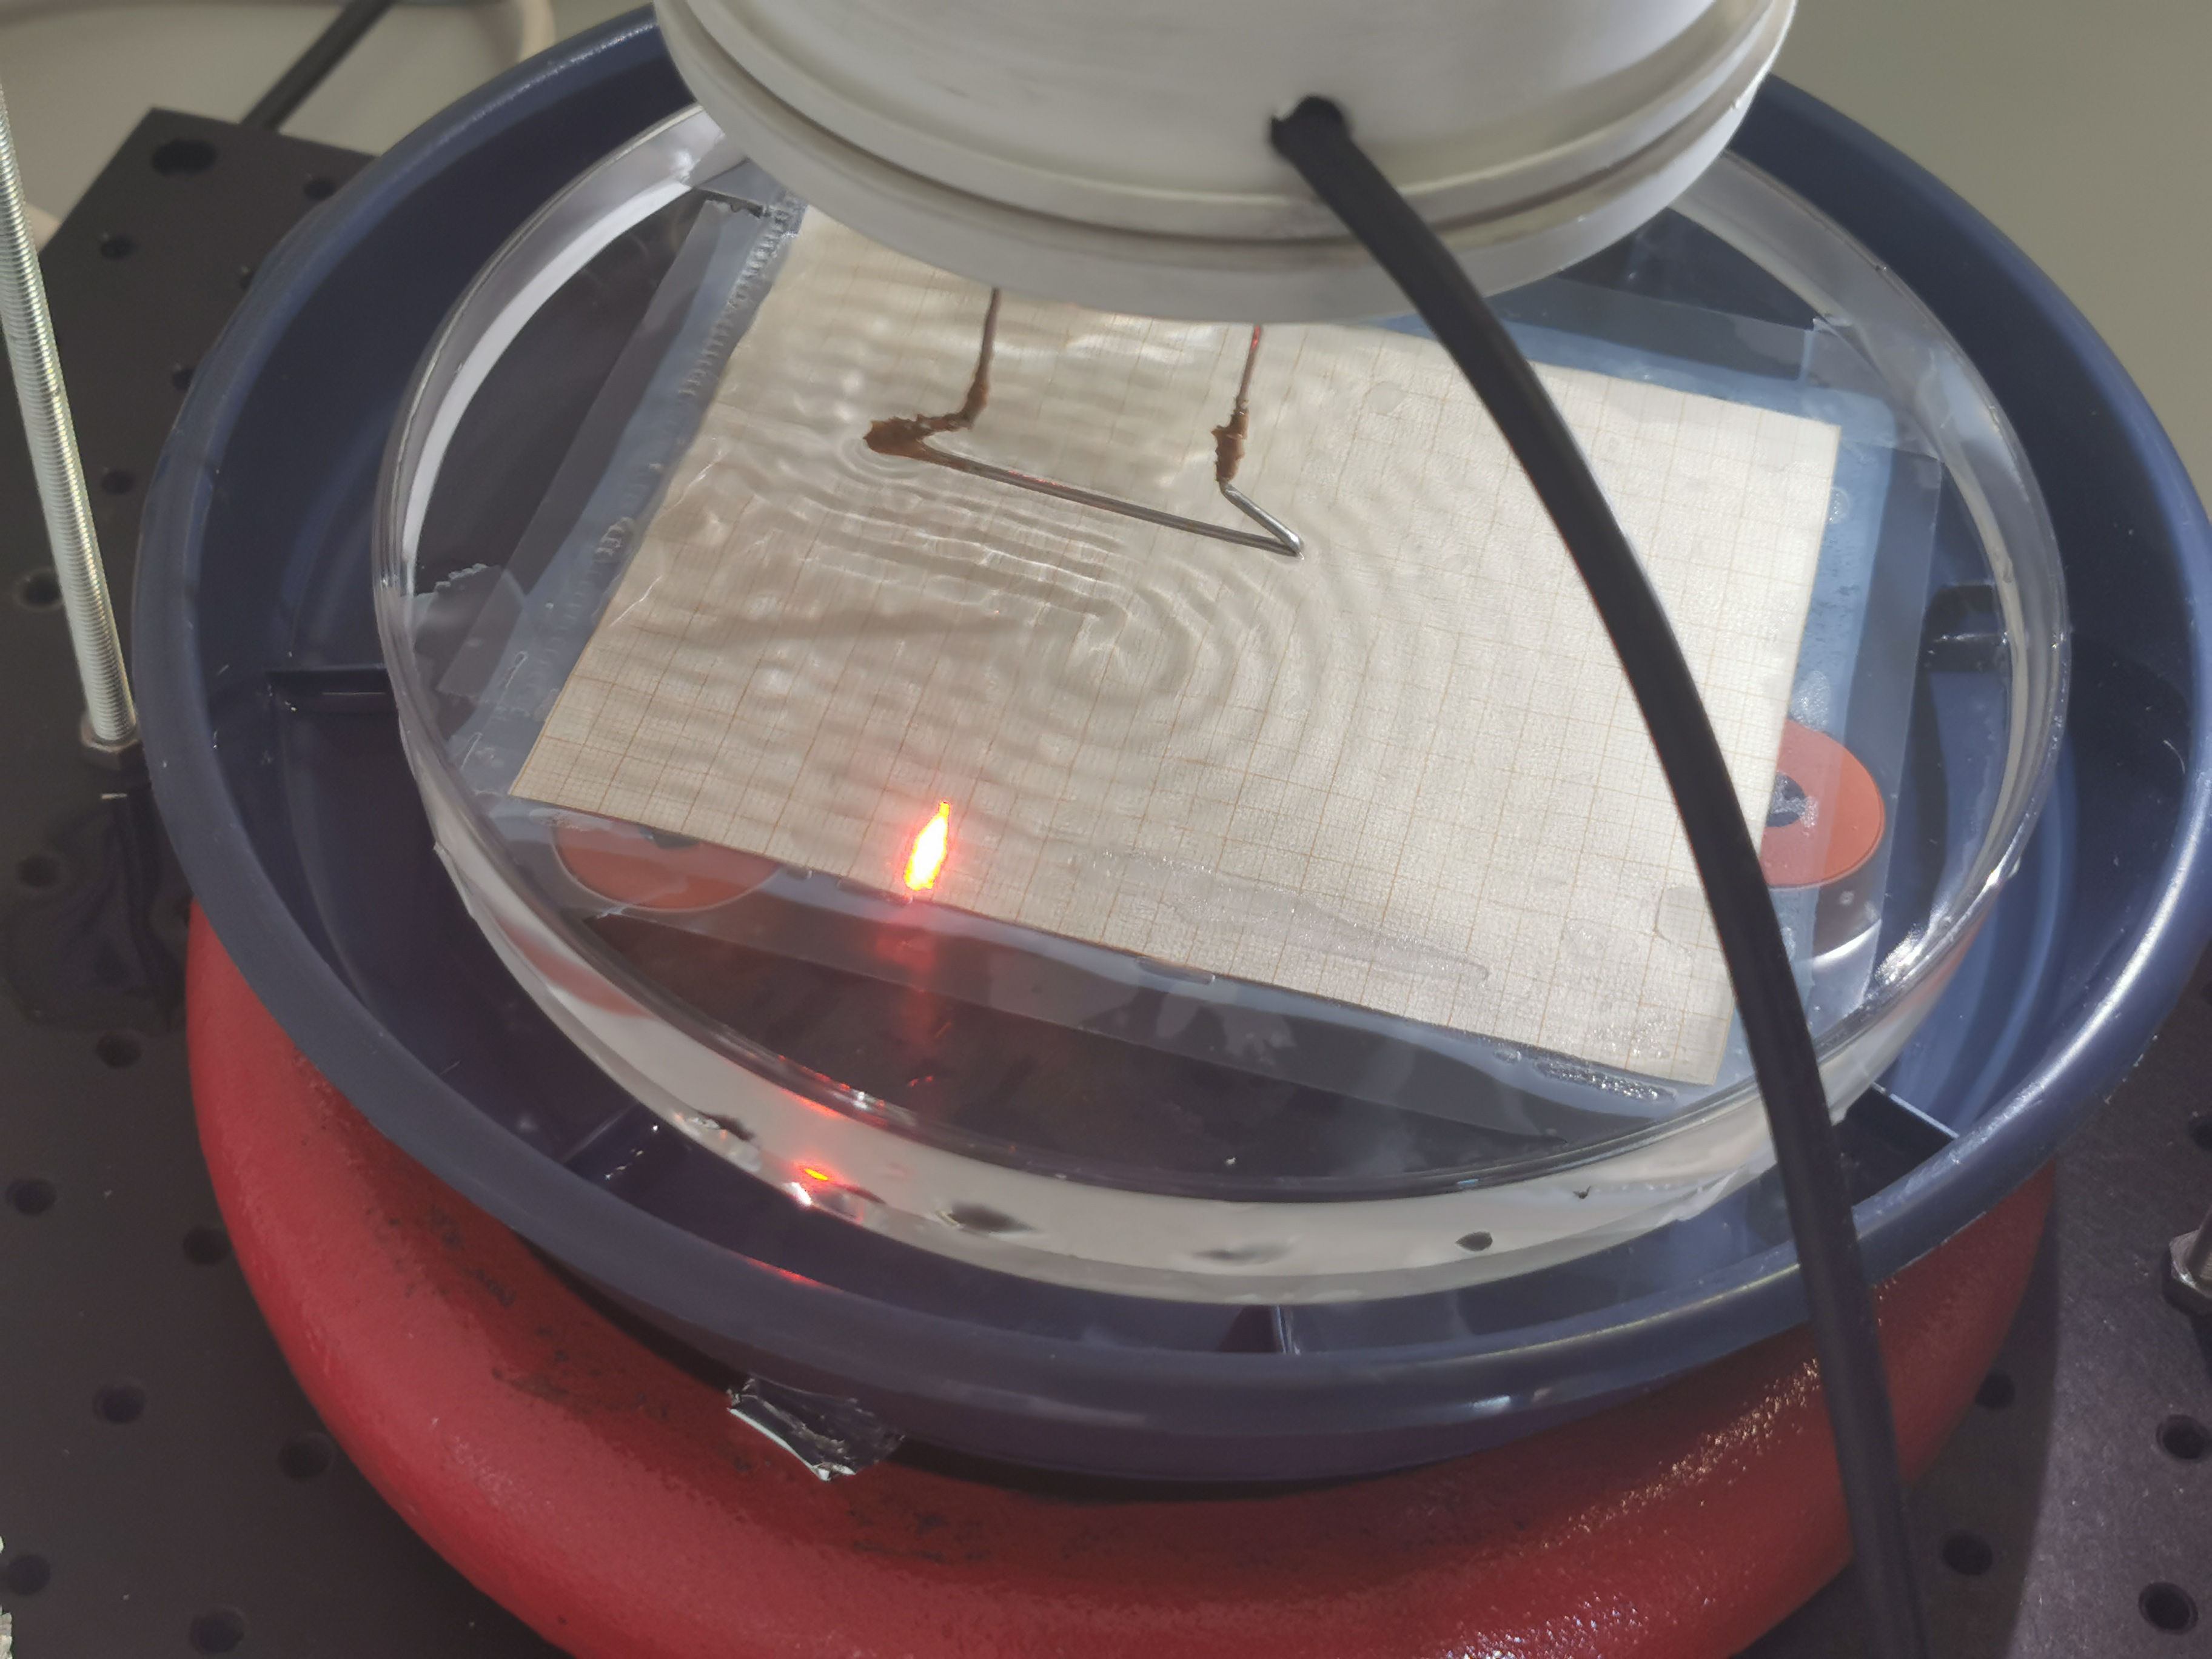
\includegraphics[width=0.6\linewidth]{../fotos/IMG_20240307_103222}
			\caption{Ondas estacionarias en la superficie}
			\label{fig:img20240307103222}
		\end{figure}
		
		\item Ajustamos el punto de incidencia del haz láser para que rebase levemente el segmento horizontal del transmisor. Nos ayudamos de una regla metálica para encontrar mejor el punto de incidencia, que nos permite comprobar por donde pasa el haz al interponerla en su recorrido. 
		
		\item Variando la amplitud de la señal, ajustamos la amplitud de la onda hasta obtener un patrón de difracción en la pantalla donde distingamos nítidamente el máximo principal y los secundarios. 
		
		\item Registramos la frecuencia y fotografiamos el patrón de difracción de la pantalla. 
		
		\item Medimos la distancia horizontal entre el punto de incidencia del láser-líquido y la pantalla. Medimos también la distancia vertical entre el punto de incidencia central en la pantalla y el punto de incidencia en el agua (altura de la superficie).
		
		\item Repetimos las mediciones en incrementos cercanos a 10 Hz para energías entre 150 y 400 Hz.
	
	\end{enumerate}
	
	
	

	
	
	\section{Tablas de medidas}
	
	
	
	\iffalse
	[Ningún misterio metodológico]
	Tabla de medidas con su pie de tabla, detallando datos. Cada tabla con su incertidumbre. tratamiento de incertidumbre de las medidas directas y la propagación de incertidumbre para las
	medidas indirectas
	Se añadirán columnas adyacentes que recojan la
	incertidumbre de las magnitudes
	 obstante, si todas las medidas presentan la
	misma incertidumbre ésta puede consignarse en la cabecera de la tabla sin
	necesidad de repetirla en cada celda de la tabla (como he hecho otras veces, vaya)
	\fi
	
	
	
	Para cada frecuencia, medimos las distancias entre máximos secundarios de primer ($c_1$) y segundo ($c_2$) orden.
	
	\begin{table}[H]
		\centering
		\begin{tabular}{|c|c|c|}
			\hline
			Frecuencia $\pm 1$ (Hz) & $c_1 \pm 1$ (mm) & $c_2 \pm 1$ (mm) \\ \hline\hline
			150                     & 13              & 26              \\ \hline
			160                     & 14              & 28              \\ \hline
			170                     & 15              & 30              \\ \hline
			180                     & 16              & 31              \\ \hline
			190                     & 16              & 32              \\ \hline
			200                     & 17              & 32              \\ \hline
			210                     & 17              & 33              \\ \hline
			220                     & 17              & 34              \\ \hline
			230                     & 17              & 35              \\ \hline
			240                     & 17              & 36              \\ \hline
			250                     & 18              & 36              \\ \hline
			260                     & 18              & 37              \\ \hline
			270                     & 19              & 39              \\ \hline
			280                     & 20              & 40              \\ \hline
			290                     & 21              & 41              \\ \hline
			300                     & 21              & 42              \\ \hline
			310                     & 21              & 42              \\ \hline
			320                     & 22              & 44              \\ \hline
			330                     & 22              & 45              \\ \hline
			340                     & 22              & 46              \\ \hline
			350                     & 23              & 48              \\ \hline
			360                     & 23              & 48              \\ \hline
			370                     & 24              & 49              \\ \hline
			380                     & 25              & 49              \\ \hline
			390                     & 25              & 50              \\ \hline
			400                     & 26              & 51              \\ \hline
		\end{tabular}
	\caption{Medidas de distancias entre centros para distintas frecuencias}
	\end{table}
	
	
	
	
	
	Tomamos las medidas de longitud del sistema:
	
	\begin{itemize}
		\item a = $4,029 \pm 0,001 \si{m}$ 
		\item b = $0,59 \pm 0,01 \si{m}$
	\end{itemize}

	\iffalse
	En ambos casos hemos trabajado con instrumentos más precisos (0,001 y 0,05), sin embargo, la medición ha sido complicada e imprecisa, ya que la altura del haz variaba con pequeñas vibraciones, y la distancia era muy larga y el punto impreciso, por este motivo hemos reducido la precisión a la estimada por nuestra toma de medidas, en lugar de la del aparato.
	\fi
	
	Con ello podemos deducir el ángulo
	\[\theta_0 = \frac{b}{a} =  0,149 \pm 0,013 
	\]
	
	donde el error ha sido propagado mediante dispersión de errores
	\[ \Delta \theta_0 = \left| \frac{\partial \theta_0}{\partial b} \right| \Delta b + \left| \frac{\partial \theta_0}{\partial a} \right| \Delta a 
	\]
	\[ \Delta \theta_0 = \frac{b}{a^2} \Delta a + \frac{1}{a} \Delta b
	\]
	\[ \theta_0 = 0,149 \pm 0,013 \text{ (rad)}
	\]

	
	Con estos datos calculamos $\omega$ y $k$ para los máximos secundarios de primer y segundo orden, así como sus errores mediante propagación de las expresiones para su cálculo
	\[\omega= 2\pi f
	\]
	\[ \Delta \omega = 2\pi \Delta f
	\]
	
	\[ k_n =\frac{\pi}{n \lambda} \frac{b c_n}{a^2}
	\]
	
	\[ \Delta k_n =  
	\frac{\pi}{n \lambda^2} \frac{b c_n}{a^2} \Delta \lambda +
	\frac{\pi}{n \lambda} \frac{ c_n}{a^2} \Delta b + 
	\frac{\pi}{n \lambda} \frac{b}{a^2} \Delta c_n +
	\frac{2\pi}{n \lambda} \frac{ b c_n}{a^3} \Delta a
	\]
	%=P5/G5*H5+P5/(M5/1000)*(1/1000) + (2*P5/$B$2)*$B$3+ (P5/$B$5)*$B$6
	
	siendo $f$ la frecuencia en herzios, $n$ el orden $\lambda$ la longitud de onda.
	
	
	
	\begin{table}[H]
		\centering
		\begin{tabular}{|c|c|c|c|c|c|}
			\hline
			Frecuencia $\pm 1$ (Hz) & $\omega \pm 6$ (rad/s) & $k_1$ (m$^{-1}$) & $\Delta k_1$ & $k_2$ (m$^{-1}$) & $\Delta k_2$ \\ \hline\hline
			150 & 942 & 2400 & 200 & 2400 & 300 \\ \hline
			160 & 1005 & 2600 & 200 & 2600 & 300 \\ \hline
			170 & 1068 & 2700 & 200 & 2700 & 300 \\ \hline
			180 & 1131 & 2900 & 200 & 2800 & 300 \\ \hline
			190 & 1194 & 2900 & 200 & 2900 & 400 \\ \hline
			200 & 1257 & 3100 & 200 & 2900 & 400 \\ \hline
			210 & 1319 & 3100 & 200 & 3000 & 400 \\ \hline
			220 & 1382 & 3100 & 200 & 3100 & 400 \\ \hline
			230 & 1445 & 3100 & 200 & 3200 & 400 \\ \hline
			240 & 1508 & 3100 & 200 & 3300 & 400 \\ \hline
			250 & 1571 & 3300 & 200 & 3300 & 400 \\ \hline
			260 & 1634 & 3300 & 200 & 3400 & 400 \\ \hline
			270 & 1696 & 3500 & 200 & 3600 & 400 \\ \hline
			280 & 1759 & 3700 & 300 & 3700 & 400 \\ \hline
			290 & 1822 & 3800 & 300 & 3800 & 400 \\ \hline
			300 & 1885 & 3800 & 300 & 3800 & 400 \\ \hline
			310 & 1948 & 3800 & 300 & 3800 & 400 \\ \hline
			320 & 2011 & 4000 & 300 & 4000 & 500 \\ \hline
			330 & 2073 & 4000 & 300 & 4100 & 500 \\ \hline
			340 & 2136 & 4000 & 300 & 4200 & 500 \\ \hline
			350 & 2199 & 4200 & 300 & 4400 & 500 \\ \hline
			360 & 2262 & 4200 & 300 & 4400 & 500 \\ \hline
			370 & 2325 & 4400 & 300 & 4500 & 500 \\ \hline
			380 & 2388 & 4600 & 300 & 4500 & 500 \\ \hline
			390 & 2450 & 4600 & 300 & 4600 & 500 \\ \hline
			400 & 2513 & 4800 & 300 & 4700 & 500 \\ \hline
		\end{tabular}
	\caption{$\omega$ y $k$ para cada frecuencia}
	\end{table}
	
	Los terceros máximos secundarios son poco visibles. Únicamente se observan con claridad en las frecuencias más altas:
	
	\begin{table}[H]
		\centering
		\begin{tabular}{|c|c|c|c|}
			\hline
			Frecuencia $\pm 1$ (Hz) & $c_3$ (mm) & $k_3$ (m$^{-1}$) & $\Delta k_3$ \\ \hline\hline
			320 & 67 & 4100 & 400 \\ \hline
			330 & 68 & 4200 & 400 \\ \hline
			340 & 69 & 4200 & 400 \\ \hline
			350 & 71 & 4300 & 400 \\ \hline
			360 & 72 & 4400 & 500 \\ \hline
			370 & 73 & 4500 & 500 \\ \hline
			380 & 74 & 4500 & 500 \\ \hline
			390 & 76 & 4600 & 500 \\ \hline
			400 & 77 & 4700 & 500 \\ \hline
		\end{tabular}
	\caption{Distancia y $k$ para máximos de tercer orden}
	\label{tab:tercerorden}
	\end{table}

	
	\section{Gráficas}
	
	\iffalse
	Pie de pagina y tabla con los datos representados. Barras de error. En ajustes lineales presentar errores y coeficiente de correlación.
	\fi
	
	Obtenemos las representaciones, para los máximos secundarios de primer y segundo orden, de $\omega^2$ frente a $k_n^3$:
	
	\subsection*{Primer orden}
	
\begin{figure}[H]
	\centering
	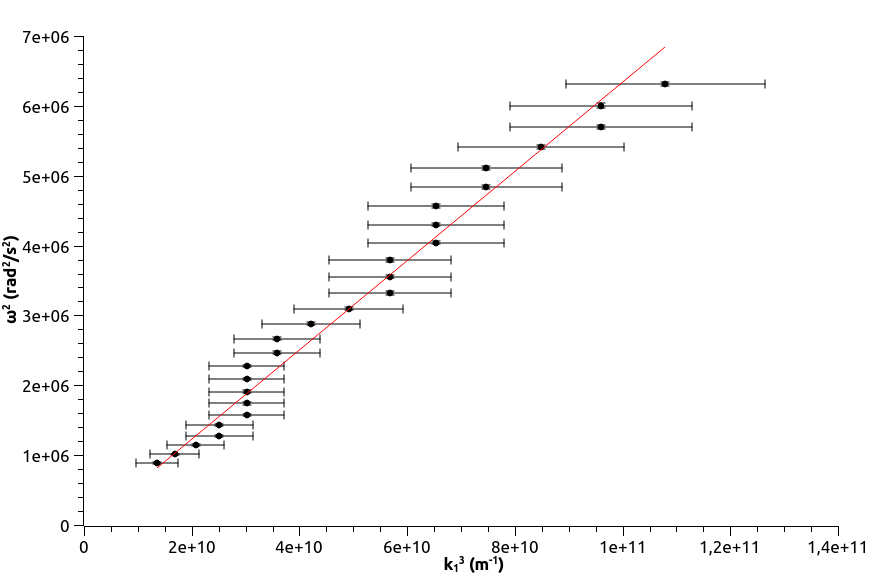
\includegraphics[width=0.9\linewidth]{../fotos/graficas/1_k13w2}
	\caption{$\omega^2$ frente a $k_1^3$, máximos secundarios de primer orden}
	\label{fig:1k13w2}
\end{figure}



% Please add the following required packages to your document preamble:
% \usepackage{longtable}
% Note: It may be necessary to compile the document several times to get a multi-page table to line up properly
\begin{longtable}[c]{|c|c|c|c|}
	\hline
	$k_1^3$ [X] & $\Delta k_1^3$ [err X] & $\omega^2$ [Y]& $\Delta \omega^2$ [err Y] \\ \hline\hline
	\endfirsthead
	%
	\endhead
	%
	1,35E+10 & 3,87E+09 & 8,88E+05 & 1,18E+04 \\ \hline
	1,69E+10 & 4,56E+09 & 1,01E+06 & 1,26E+04 \\ \hline
	2,07E+10 & 5,31E+09 & 1,14E+06 & 1,34E+04 \\ \hline
	2,52E+10 & 6,13E+09 & 1,28E+06 & 1,42E+04 \\ \hline
	2,52E+10 & 6,13E+09 & 1,43E+06 & 1,50E+04 \\ \hline
	3,02E+10 & 7,02E+09 & 1,58E+06 & 1,58E+04 \\ \hline
	3,02E+10 & 7,02E+09 & 1,74E+06 & 1,66E+04 \\ \hline
	3,02E+10 & 7,02E+09 & 1,91E+06 & 1,74E+04 \\ \hline
	3,02E+10 & 7,02E+09 & 2,09E+06 & 1,82E+04 \\ \hline
	3,02E+10 & 7,02E+09 & 2,27E+06 & 1,89E+04 \\ \hline
	3,58E+10 & 7,99E+09 & 2,47E+06 & 1,97E+04 \\ \hline
	3,58E+10 & 7,99E+09 & 2,67E+06 & 2,05E+04 \\ \hline
	4,21E+10 & 9,02E+09 & 2,88E+06 & 2,13E+04 \\ \hline
	4,91E+10 & 1,01E+10 & 3,10E+06 & 2,21E+04 \\ \hline
	5,69E+10 & 1,13E+10 & 3,32E+06 & 2,29E+04 \\ \hline
	5,69E+10 & 1,13E+10 & 3,55E+06 & 2,37E+04 \\ \hline
	5,69E+10 & 1,13E+10 & 3,79E+06 & 2,45E+04 \\ \hline
	6,54E+10 & 1,26E+10 & 4,04E+06 & 2,53E+04 \\ \hline
	6,54E+10 & 1,26E+10 & 4,30E+06 & 2,61E+04 \\ \hline
	6,54E+10 & 1,26E+10 & 4,56E+06 & 2,68E+04 \\ \hline
	7,47E+10 & 1,40E+10 & 4,84E+06 & 2,76E+04 \\ \hline
	7,47E+10 & 1,40E+10 & 5,12E+06 & 2,84E+04 \\ \hline
	8,49E+10 & 1,54E+10 & 5,40E+06 & 2,92E+04 \\ \hline
	9,60E+10 & 1,69E+10 & 5,70E+06 & 3,00E+04 \\ \hline
	9,60E+10 & 1,69E+10 & 6,00E+06 & 3,08E+04 \\ \hline
	1,08E+11 & 1,85E+10 & 6,32E+06 & 3,16E+04 \\ \hline
	\caption{Tabla de datos de la Figura \ref{fig:1k13w2}}
\end{longtable}

\iffalse
[viernes, 19 de abril de 2024 18:24:27 (CEST)	Gráfica: ''Gráfica5'']
Regresión Lineal ajuste del conjunto de datos: Tabla1_w^2, usando función : A*x+B
errores estándar Y: conjunto de datos asociados (Tabla1_error w^2)
Desde x = 13.494.767.538,7705 a x = 107.958.140.310,164
B (y-intercección) = -46.317,5221053134 +/- 7.301,92426602887
A (pendiente) = 6,38526856049185e-05 +/- 1,69027863606673e-07
--------------------------------------------------------------------------------------
Chi^2 = 3.482,06849835592
R^2 = 0,976180871259703
---------------------------------------------------------------------------------------

\fi

La recta de ajuste para la Figura \ref{fig:1k13w2}:

\[ \omega^2 = k^3 x +B
\]
\[A = (6,385 \pm 0,017) \cdot 10^{-5} \si{(rad\cdot m/s)}  %A (pendiente) = 6,38526856049185e-05 +/- 1,69027863606673e-07
\]
\[ B = (-46000\pm 7000)\si{(m/s)}
\]
Siendo la correlación:
\[ R^2 =  0,9762
\]

\subsection*{Segundo orden}

\begin{figure}[H]
	\centering
	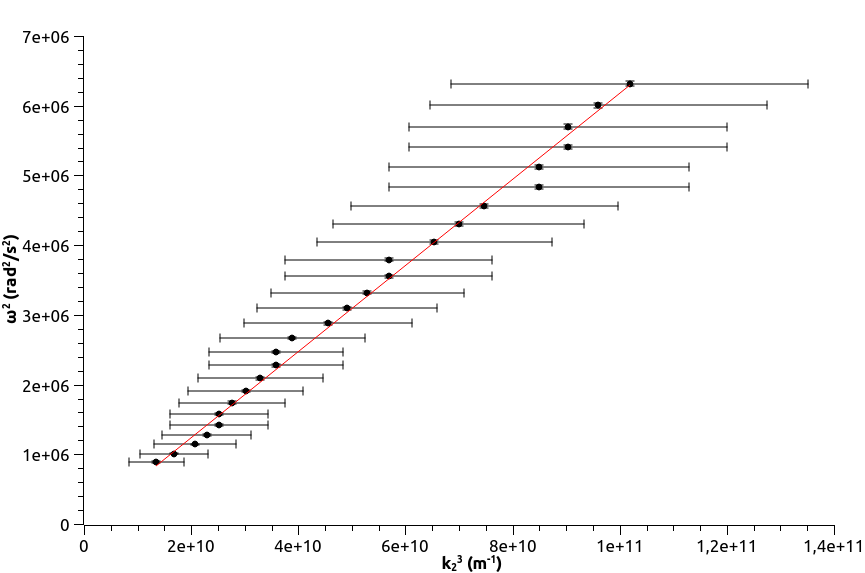
\includegraphics[width=0.9\linewidth]{../fotos/graficas/1_k23w2}
	\caption{$\omega^2$ frente a $k_2^3$, máximos secundarios de segundo orden}
	\label{fig:1k23w2}
\end{figure}


	
	% Please add the following required packages to your document preamble:
	% \usepackage{longtable}
	% Note: It may be necessary to compile the document several times to get a multi-page table to line up properly
	\begin{longtable}[c]{|c|c|c|c|}
		\hline
		$k_1^3$ [X] & $\Delta k_1^3$ [err X] & $\omega^2$ [Y] & $\Delta \omega^2$ [err Y] \\ \hline
		\endfirsthead
		%
		\endhead
		%
		1,35E+10 & 5,17E+09 & 8,88E+05 & 1,18E+04 \\ \hline
		1,69E+10 & 6,32E+09 & 1,01E+06 & 1,26E+04 \\ \hline
		2,07E+10 & 7,62E+09 & 1,14E+06 & 1,34E+04 \\ \hline
		2,29E+10 & 8,34E+09 & 1,28E+06 & 1,42E+04 \\ \hline
		2,52E+10 & 9,10E+09 & 1,43E+06 & 1,50E+04 \\ \hline
		2,52E+10 & 9,10E+09 & 1,58E+06 & 1,58E+04 \\ \hline
		2,76E+10 & 9,90E+09 & 1,74E+06 & 1,66E+04 \\ \hline
		3,02E+10 & 1,07E+10 & 1,91E+06 & 1,74E+04 \\ \hline
		3,29E+10 & 1,16E+10 & 2,09E+06 & 1,82E+04 \\ \hline
		3,58E+10 & 1,26E+10 & 2,27E+06 & 1,89E+04 \\ \hline
		3,58E+10 & 1,26E+10 & 2,47E+06 & 1,97E+04 \\ \hline
		3,89E+10 & 1,36E+10 & 2,67E+06 & 2,05E+04 \\ \hline
		4,55E+10 & 1,57E+10 & 2,88E+06 & 2,13E+04 \\ \hline
		4,91E+10 & 1,68E+10 & 3,10E+06 & 2,21E+04 \\ \hline
		5,29E+10 & 1,80E+10 & 3,32E+06 & 2,29E+04 \\ \hline
		5,69E+10 & 1,93E+10 & 3,55E+06 & 2,37E+04 \\ \hline
		5,69E+10 & 1,93E+10 & 3,79E+06 & 2,45E+04 \\ \hline
		6,54E+10 & 2,20E+10 & 4,04E+06 & 2,53E+04 \\ \hline
		7,00E+10 & 2,34E+10 & 4,30E+06 & 2,61E+04 \\ \hline
		7,47E+10 & 2,49E+10 & 4,56E+06 & 2,68E+04 \\ \hline
		8,49E+10 & 2,80E+10 & 4,84E+06 & 2,76E+04 \\ \hline
		8,49E+10 & 2,80E+10 & 5,12E+06 & 2,84E+04 \\ \hline
		9,03E+10 & 2,97E+10 & 5,40E+06 & 2,92E+04 \\ \hline
		9,03E+10 & 2,97E+10 & 5,70E+06 & 3,00E+04 \\ \hline
		9,60E+10 & 3,15E+10 & 6,00E+06 & 3,08E+04 \\ \hline
		1,02E+11 & 3,33E+10 & 6,32E+06 & 3,16E+04 \\ \hline
		\caption{Tabla de datos de la Figura \ref{fig:1k23w2}}
	\end{longtable}
	
	\iffalse
	
	[viernes, 19 de abril de 2024 18:36:19 (CEST)	Gráfica: ''Gráfica6'']
	Regresión Lineal ajuste del conjunto de datos: Tabla2_k2^3, usando función : A*x+B
	errores estándar Y: conjunto de datos asociados (Tabla2_w^2)
	Desde x = 13.494.767.538,7705 a x = 101.848.794.309,595
	B (y-intercección) = 4.911,68682648754 +/- 7.143,33620676411
	A (pendiente) = 6,17664884672444e-05 +/- 1,62170756576638e-07
	--------------------------------------------------------------------------------------
	Chi^2 = 1.123,53991878176
	R^2 = 0,992314412544451
	---------------------------------------------------------------------------------------
	\fi
	
	
	
	La recta de ajuste para la Figura \ref{fig:1k23w2}:
	
	\[ \omega^2 = k^3 x +B
	\]
	\[A = (6,177 \pm 0,016) \cdot 10^{-5} \si{(rad\cdot m/s)}%6,17664884672444e-05 +/- 1,62170756576638e-07
	\]
	\[ B = (-5000\pm 7000)\si{(m/s)}    %4.911,68682648754 +/- 7.143,33620676411
	\]
	Siendo la correlación:
	\[ R^2 =  0,9923
	\]
	
	\subsection*{Tercer orden}
	
	A partir de la Tabla \ref{tab:tercerorden}, graficamos la parte de la recta obtenida por esos datos:
	
\begin{figure}[H]
	\centering
	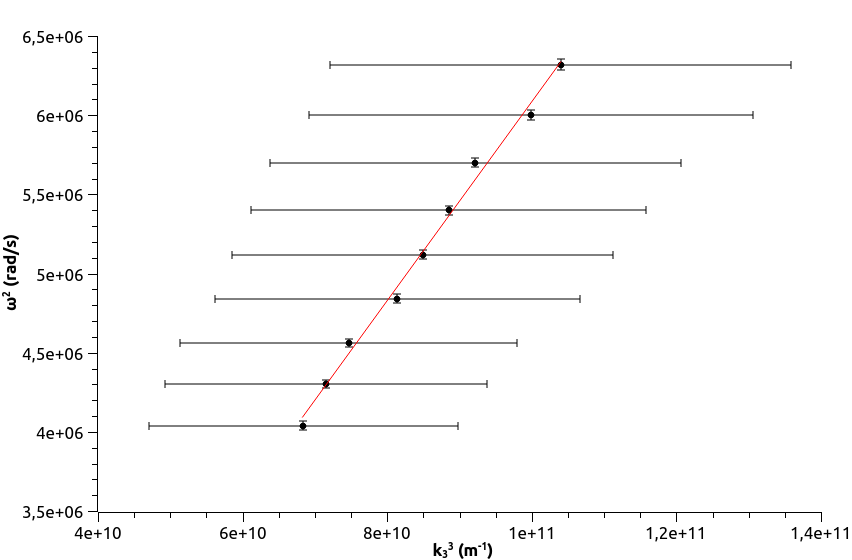
\includegraphics[width=0.9\linewidth]{../fotos/graficas/1_k33w2}
	\caption{}
	\label{fig:1k33w2}
	\caption{$\omega^2$ frente a $k_3^3$, máximos secundarios de tercer orden}
\end{figure}
	
	\begin{table}[H]
		\centering
		\begin{tabular}{|c|c|c|c|}\hline
			$k_3^3$ [X] & $\Delta k_3^3$ [err X] & $\omega^2$ [Y] & $\Delta \omega^2$ [err Y] \\ \hline
			6,84E+10 & 2,14E+10 & 4,04E+06 & 2,53E+04 \\\hline
			7,15E+10 & 2,23E+10 & 4,30E+06 & 2,61E+04 \\\hline
			7,47E+10 & 2,33E+10 & 4,56E+06 & 2,68E+04 \\\hline
			8,14E+10 & 2,52E+10 & 4,84E+06 & 2,76E+04 \\\hline
			8,49E+10 & 2,63E+10 & 5,12E+06 & 2,84E+04 \\\hline
			8,85E+10 & 2,73E+10 & 5,40E+06 & 2,92E+04 \\\hline
			9,22E+10 & 2,84E+10 & 5,70E+06 & 3,00E+04 \\\hline
			9,99E+10 & 3,07E+10 & 6,00E+06 & 3,08E+04 \\\hline
			1,04E+11 & 3,19E+10 & 6,32E+06 & 3,16E+04\\ \hline
		\end{tabular}
	\caption{Tabla de datos para la Figura \ref{fig:1k33w2}}
	\end{table}

	
	La recta de ajuste para la Figura \ref{fig:1k23w2}:
	
	\[ \omega^2 = k^3 x +B
	\]
	\[A = (6,30 \pm 0,08) \cdot 10^{-5} \si{(rad\cdot m/s)}       %6,29839472950103e-05 +/- 8,16135427569135e-07
	\]
	\[ B = (-220000\pm 70000)\si{(m/s)}    
	\]
	Siendo la correlación:
	\[ R^2 =  0,9934
	\]

%% -215.592,181355195 +/- 68.711,8901196626
	
	
	\section{Discusión de resultados}
	
	\iffalse
	Cuestiones. 
	Justificación de los resultados. 
	Comparativa de los valores experimentales obtenidos con los publicados en la literatura (?!?!)
	Posibles fuentes de incertidumbre que expliquen la discrepancia.
	\fi
	
	A partir de 
	\[ \omega^2 = \frac{\sigma}{\rho} k^3 \longrightarrow \sigma = \frac{\omega^2}{k^3}\rho
	\]
	\[ \Delta \sigma = \frac{2\omega}{k^3}\rho \Delta \omega + \frac{3\omega^2}{k^4}\rho\Delta k + \frac{\omega^2}{k^3}\Delta \rho
	\]
	
	
	Utilizando la relación de dispersión de los máximos secundarios de primer orden, y conociendo la densidad del agua:
	\[ \frac{\omega^2}{k^3} = (6,385 \pm 0,017) \cdot 10^{-5} \si{(rad\cdot m/s)} 
	\]
	\[\rho_{agua} = 977\pm 1\si{(kg/m^3)}
	\]
	\[ \sigma_1 = \frac{\omega^2}{k^3} \rho_{agua}= (62,4\pm 0,2)\cdot 10^{-3}\si{(N/m)}
	\]
	% tengo mucho lío aquí con las unidades
	
	
	%  72,8 milinewtons (mN) por metro a 20 °C
	
	Si utilizamos los máximos secundarios de segundo y tercer orden
	
	\[ \sigma_2 = \frac{\omega^2}{k^3}\rho_{agua} = (60,3\pm 0,2)\cdot 10^{-3} \si{(N/m)} %(6,177 \pm 0,016) \cdot 10^{-5}
	\]
	\[ \sigma_3 = \frac{\omega^2}{k^3}\rho_{agua} = (61,6\pm 0,8)\cdot 10^{-3} \si{(N/m)} 
	\]
	
	
	
	%[cambiar la precisión de las medidas]\\
	
	%[comparar con la literatura]\\
	
	Según la literatura, el valor de la tensión superficial del agua a 20ºC es de 
	\[\sigma_{teor} = (72,8\pm 0,1)\cdot 10^{-3} \si{N/m} \]
	
	La diferencia entre nuestros valores de $\sigma$ calculados y el teórico es considerable, de más de un 17\%, incluso para los máximos secundarios de tercer orden, para los que posiblemente no disponemos de suficientes puntos. Entre las posibles causas de error, las mediciones de distancias $a$ y $b$ resultaban complicadas, tanto por la gran distancia que cubría $a$ como por la oscilación en altura de $b$ y la dificultad determinando el punto de reflexión del haz en el agua. Además, las ondas en el agua se veían fácilmente perturbadas por las vibraciones en la sala. 
	
	%[explicar que esas las medidas con regla eran extremadamente imprecisas y todo lo que se movía el aparato]\\
	
	
	
	%[comparar la magnitud de la fuerza por volumen de las gravedad (rho * g) y ondas superficiales (sigma * k$^2$), número de onda crítico a partir del que se tienen en cuenta los efectos de gravedad. Comparar con los k experimental]
	
	%rho*g 
	
	\subsection*{Número de onda crítico}
	
	\[g = 9,81\pm0,01 \si{N/kg}\]
	
	\[\rho \cdot g = 9580\pm 20\si{N/m^3}\]
	
	Comparando con la fuerza de las ondas superficiales, podemos despejar un número de onda crítico, en el que ambas fuerzas se igualan
	\[ \sigma \cdot k^2 = \rho \cdot g \longrightarrow k = \sqrt{\frac{\rho \cdot g}{\sigma}}
	\]
	\[ \Delta k = \frac{1}{2}\sqrt{\frac{g}{\sigma \cdot \rho}} \Delta \rho +  \frac{1}{2}\sqrt{\frac{\rho}{\sigma \cdot g}} \Delta g + \frac{1}{2}\sqrt{\frac{\rho \cdot g}{\sigma^3}} \Delta\sigma
	\]
	
	
	Utilizando el valor teórico $\sigma_{teor}$
	\[ k_c = (362,8 \pm 0,6) \si{m^{-1}}
	\]
	Mientras que utilizando nuestro valor experimental $\sigma_2$
	\[ k_c = (398\pm 1)\si{m^{-1}}
	\]
	
	
	Esto indica el número de onda crítico a partir del que los efectos de la gravedad son significativos respecto a los de la tensión superficial, es un orden de magnitud más bajo que el rango en el que nos hemos movido.
	
	
	
	
	
	\section{Conclusiones}
	
	
	%Lo típico
	
	Mediante la medida de las distancias en un patrón de difracción sobre ondas de tensión superficial estacionarias generadas a partir de la frecuencia emitida por un altavoz sobre la superficie de agua, hemos podido determinar la relación entre el número de onda y su velocidad angular, y con ello obtener una medida experimental de la tensión superficial del agua. La disposición del experimento y la dificultad de algunas de las medidas han reducido la precisión de los resultados considerablemente.
	
	
	
	
	
	
	
	
	
	
	
	
\end{document}